%----------createAssociationEndIsClass----------------------------------------
\op
{createAssociationEndIsClass}
{Creates a new association end under the selected association and links it to a
class that lies in the same package as the association}
{createAssociationEndIsClass(Association
selectedEObject, String nameValue, String idValue, String srcMultiplicity)} {The
association providing the container for the newly created association end.} {
\begin{itemize}
 \item nameValue/newName: The name of the newly created association end
 \item idValue/newID: The id of the newly created association end
 \item srcMultiplicity/newMultiplicity: The multiplicity of the newly created
 source association end
\end{itemize}
}
{There mustn't be an association end under the selected association with the
same name like in 'newName' (see
\ref{subsec:checkOtherNames})}
{Only the name, id and multiplicity will be set via input data. isNavigable,
kind and isOrdered will be set with a default value as defined with the diagram
editor in the image below.
Note that the reference from a class and from the selected association point to
the same unknown package. This will make sure that there won't be created
associations between classes of different packages.}
\begin{figure}[H]
  \centering
  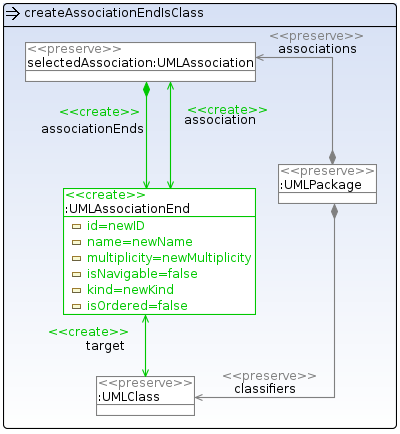
\includegraphics[width=0.65\textwidth]{pics/createAssociationEndIsClass.png}
  \caption{createAssociationEndIsClass}
  \label{createAssociationEndIsClass}
\end{figure}
%----------createAssociationEndIsInterface----------------------------------------
\op
{createAssociationEndIsInterface}
{Creates a new association end under the selected association and links it to an
interface that lies in the same package as the association}
{createAssociationEndIsInterface(Association
selectedEObject, String nameValue, String idValue, String srcMultiplicity)} {The
association providing the container for the newly created association end.} {
\begin{itemize}
 \item nameValue/newName: The name of the newly created association end
 \item idValue/newID: The id of the newly created association end
 \item srcMultiplicity/newMultiplicity: The multiplicity of the newly created
 source association end
\end{itemize}
}
{There mustn't be an association end under the selected association with the
same name like in 'newName' (see
\ref{subsec:checkOtherNames})}
{Only the name, id and multiplicity will be set via input data. isNavigable,
kind and isOrdered will be set with a default value as defined with the diagram
editor in the image below.
Note that the reference from an interface and from the selected association
point to the same unknown package. This will make sure that there won't be created
associations between interfaces of different packages.}
\begin{figure}[H]
  \centering
  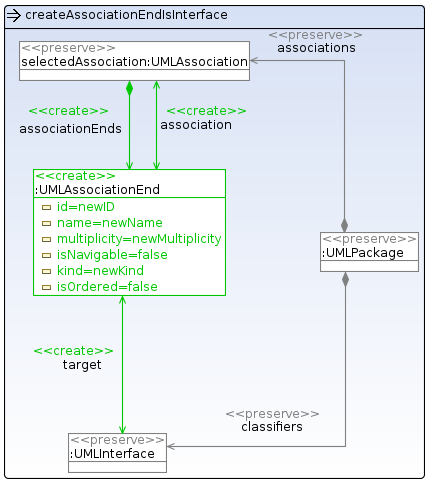
\includegraphics[width=0.65\textwidth]{pics/createAssociationEndIsInterface.png}
  \caption{createAssociationEndIsInterface}
  \label{createAssociationEndIsInterface}
\end{figure}
%----------deleteAssociationEnd----------------------------------------
\op
{deleteAssociationEnd}
{Deletes an association end and the reference to its actuall target, but not
the target itself}
{deleteAssociationEnd(AssociationEnd selectedEObject)}
{The association end which should be deleted including its reference}
{-}
{-}
{This transformation is designed with three rules. The first two rules will
delete an association end depending on which type it points to. The third one
will simply do nothing but is still required in the TransformationUnits.
\\\\You can see that the 'mainUnit' is a Conditional Unit this time. It will try to
run the rule 'deleteAssociationEndIsClass' and in case it will match this
means that the modification has worked and there is nothing left to do (that's
why a 'doNothing-Rule' is following in the 'Then'-part). Otherwise, if our
selected association end does not point to a class, we assume that it can only point to
an interface and therefore 'deleteAssociationEndIsInterface' will be called.
}
\begin{figure}[H]
  \centering
  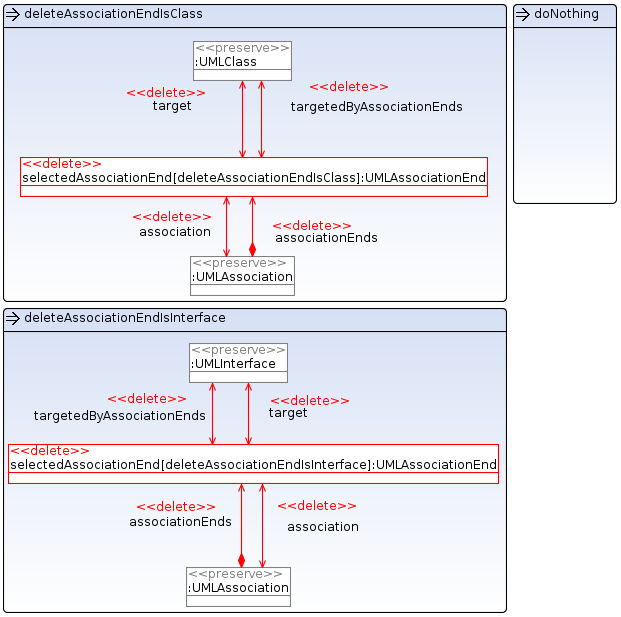
\includegraphics[width=0.8\textwidth]{pics/deleteAssociationEnd.png}
  \caption{deleteAssociationEnd}
  \label{deleteAssociationEnd}
\end{figure}
\begin{figure}[H]
  \centering
  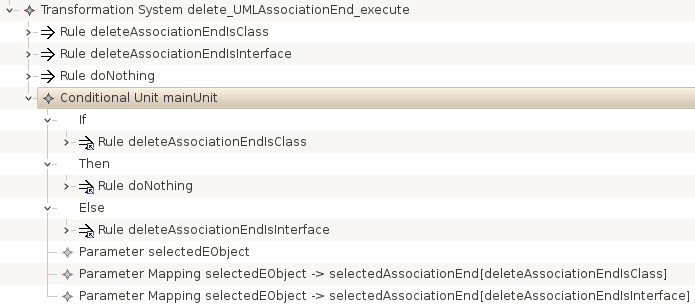
\includegraphics[width=1.0\textwidth]{pics/deleteAssociationEnd_TreeView.png}
  \caption{deleteAssociationEnd(UnitView)}
  \label{deleteAssociationEnd(UnitView)}
\end{figure}
%----------editAssociationEndFromClassToClass----------------------------------------
\op
{editAssociationEndFromClassToClass}
{Edits the target of an association end to another class}
{editAssociationEndFromClassToClass(AssociationEnd selectedEObject, Class
tgt)}
{The association end whose target should be changed}
{
\begin{itemize}
 \item tgt/targetClass: The new class
\end{itemize}
}
{-}
{Only references will change.}
\begin{figure}[H]
  \centering
  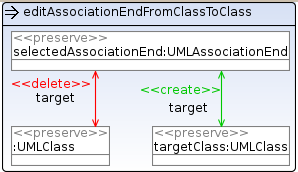
\includegraphics[width=0.4\textwidth]{pics/editAssociationEndFromClassToClass.png}
  \caption{editAssociationEndFromClassToClass}
  \label{editAssociationEndFromClassToClass}
\end{figure}
%----------editAssociationEndFromClassToInterface----------------------------------------
\op
{editAssociationEndFromClassToInterface}
{Edits the target of an association end from a class to an interface}
{editAssociationEndFromClassToInterface(AssociationEnd selectedEObject,
Interface tgt)}
{The association end whose target should be changed}
{
\begin{itemize}
 \item tgt/targetInterface: The new interface
\end{itemize}
}
{-}
{Only references will change.}
\begin{figure}[H]
  \centering
  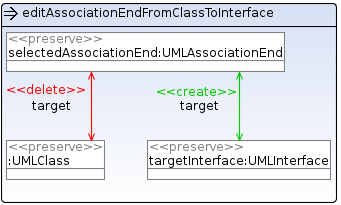
\includegraphics[width=0.45\textwidth]{pics/editAssociationEndFromClassToInterface.png}
  \caption{editAssociationEndFromClassToInterface}
  \label{editAssociationEndFromClassToInterface}
\end{figure}
%----------editAssociationEndFromInterfaceToClass----------------------------------------
\op
{editAssociationEndFromInterfaceToClass}
{Edits the target of an association end from an interface to a class}
{editAssociationEndFromInterfaceToClass(AssociationEnd selectedEObject,
Class tgt)}
{The association end whose target should be changed}
{
\begin{itemize}
 \item tgt/targetClass: The new class
\end{itemize}
}
{-}
{Only references will change.}
\begin{figure}[H]
  \centering
  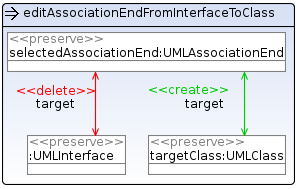
\includegraphics[width=0.4\textwidth]{pics/editAssociationEndFromInterfaceToClass.png}
  \caption{editAssociationEndFromInterfaceToClass}
  \label{editAssociationEndFromInterfaceToClass}
\end{figure}
%----------editAssociationEndFromInterfaceToInterface----------------------------------------
\op
{editAssociationEndFromInterfaceToInterface}
{Edits the target of an association end to another interface}
{editAssociationEndFromInterfaceToInterface(AssociationEnd selectedEObject,
Interface tgt)}
{The association end whose target should be changed}
{
\begin{itemize}
 \item tgt/targetInterface: The new interface
\end{itemize}
}
{-}
{Only references will change.}
\begin{figure}[H]
  \centering
  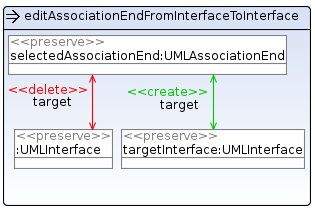
\includegraphics[width=0.45\textwidth]{pics/editAssociationEndFromInterfaceToInterface.png}
  \caption{editAssociationEndFromInterfaceToInterface}
  \label{editAssociationEndFromInterfaceToInterface}
\end{figure}
%----------editAssociationEndIsNavigatable----------------------------------------
\op
{editAssociationEndIsNavigatable}
{Edits the isNavigatable-value of an association end}
{editAssociationEndIsNavigatable(AssociationEnd selectedEObject, boolean
booleanValue)}
{The association end whose isNavigatable-value should be edited.}
{
\begin{itemize}
 \item booleanValue/bool: The new isNavigatable-value
\end{itemize}
}
{-}
{The \textless\textless create\textgreater\textgreater  -symbol in the image
means that even if the attribute exists its value will be overwritten.
'bool' is the placeholder for the input bool value.}
\begin{figure}[H]
  \centering
  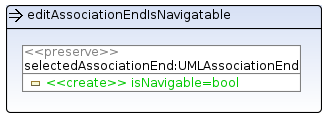
\includegraphics[width=0.45\textwidth]{pics/editAssociationEndIsNavigatable.png}
  \caption{editAssociationEndIsNavigatable}
  \label{editAssociationEndIsNavigatable}
\end{figure}
%----------editAssociationEndIsOrdered----------------------------------------
\op
{editAssociationEndIsOrdered}
{Edits the isOrdered-value of an association end}
{editAssociationEndIsOrdered(AssociationEnd selectedEObject, boolean
booleanValue)}
{The association end whose isOrdered-value should be edited.}
{
\begin{itemize}
 \item booleanValue/bool: The new isOrdered-value
\end{itemize}
}
{-}
{The \textless\textless create\textgreater\textgreater  -symbol in the image
means that even if the attribute exists its value will be overwritten.
'bool' is the placeholder for the input bool value.}
\begin{figure}[H]
  \centering
  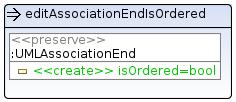
\includegraphics[width=0.4\textwidth]{pics/editAssociationEndIsOrdered.png}
  \caption{editAssociationEndIsOrdered}
  \label{editAssociationEndIsOrdered}
\end{figure}
%----------editAssociationEndName----------------------------------------
\op
{editAssociationEndName}
{Edits the name of an association end}
{editAssociationEndName(AssociationEnd selectedEObject, String nameValue)}
{The class whose name should be renamed.}
{
\begin{itemize}
 \item nameValue/newName: The new name
\end{itemize}
}
{There is no association end under the same association whose name equals the
parameter-value of 'newName' (see
\ref{subsec:checkOtherNames})}
{The \textless\textless create\textgreater\textgreater  -symbol in the image
means that even if the attribute exists its value will be overwritten.
'newName' is the placeholder for the input name.}
\begin{figure}[H]
  \centering
  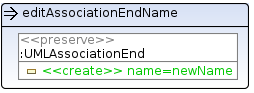
\includegraphics[width=0.4\textwidth]{pics/editAssociationEndName.png}
  \caption{editAssociationEndName}
  \label{editAssociationEndName}
\end{figure}
%----------editAssociationEndKind----------------------------------------
\op
{editAssociationEndKind}
{Edits the kind (none, shared or composit) of an association end}
{editAssociationEndKind(AssociationEnd selectedEObject, Kind kindValue)}
{The class whose name should be renamed.}
{
\begin{itemize}
 \item kindValue/newKind: The new kind
\end{itemize}
}
{The opposit ending mustn't also be composit if the new kind is composit
(see
\ref{subsec:checkOppositeAggregationKind})}
{The \textless\textless create\textgreater\textgreater  -symbol in the image
means that even if the attribute exists its value will be overwritten.
'newKind' is the placeholder for the input kind value.}
\begin{figure}[H]
  \centering
  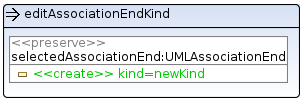
\includegraphics[width=0.45\textwidth]{pics/editAssociationEndKind.png}
  \caption{editAssociationEndKind}
  \label{editAssociationEndKind}
\end{figure}
%----------editAssociationEndMultiplicity----------------------------------------
\op
{editAssociationEndMultiplicity}
{Edits the multiplicity of an association end}
{editAssociationEndMultiplicity(AssociationEnd selectedEObject, String
srcMultiplicity)}
{The class whose name should be renamed.}
{
\begin{itemize}
 \item srcMultiplicity/newMultiplicity: The new multiplicity
\end{itemize}
}
{-}
{The \textless\textless create\textgreater\textgreater  -symbol in the image
means that even if the attribute exists its value will be overwritten.
'newMultiplicity' is the placeholder for the input multiplicity value.}
\begin{figure}[H]
  \centering
  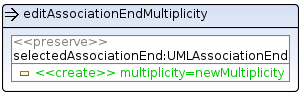
\includegraphics[width=0.45\textwidth]{pics/editAssociationEndMultiplicity.png}
  \caption{editAssociationEndMultiplicity}
  \label{editAssociationEndMultiplicity}
\end{figure}